\begin{figure}[htb!]
\centering
\begin{tabular}{lll}
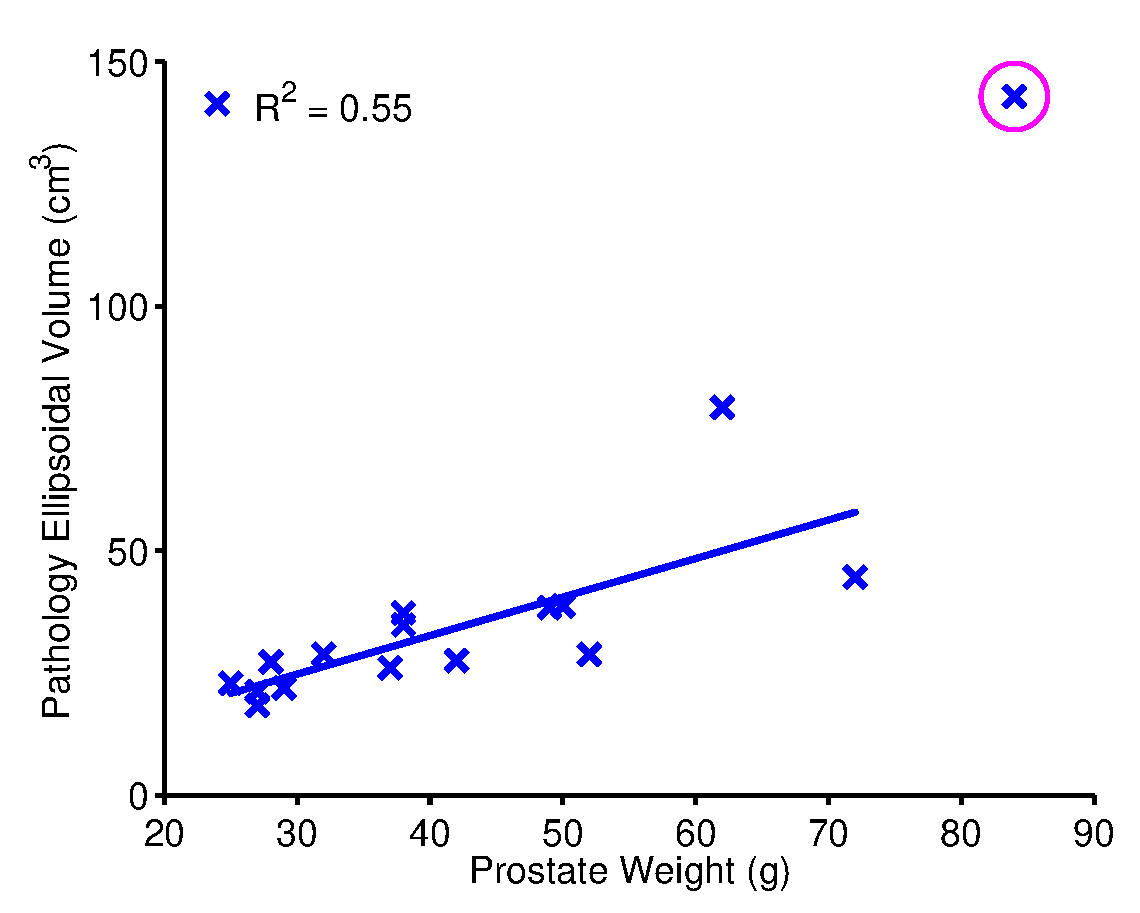
\includegraphics[width=0.3\linewidth]{figs/corr_path_vol_weight_vol} &
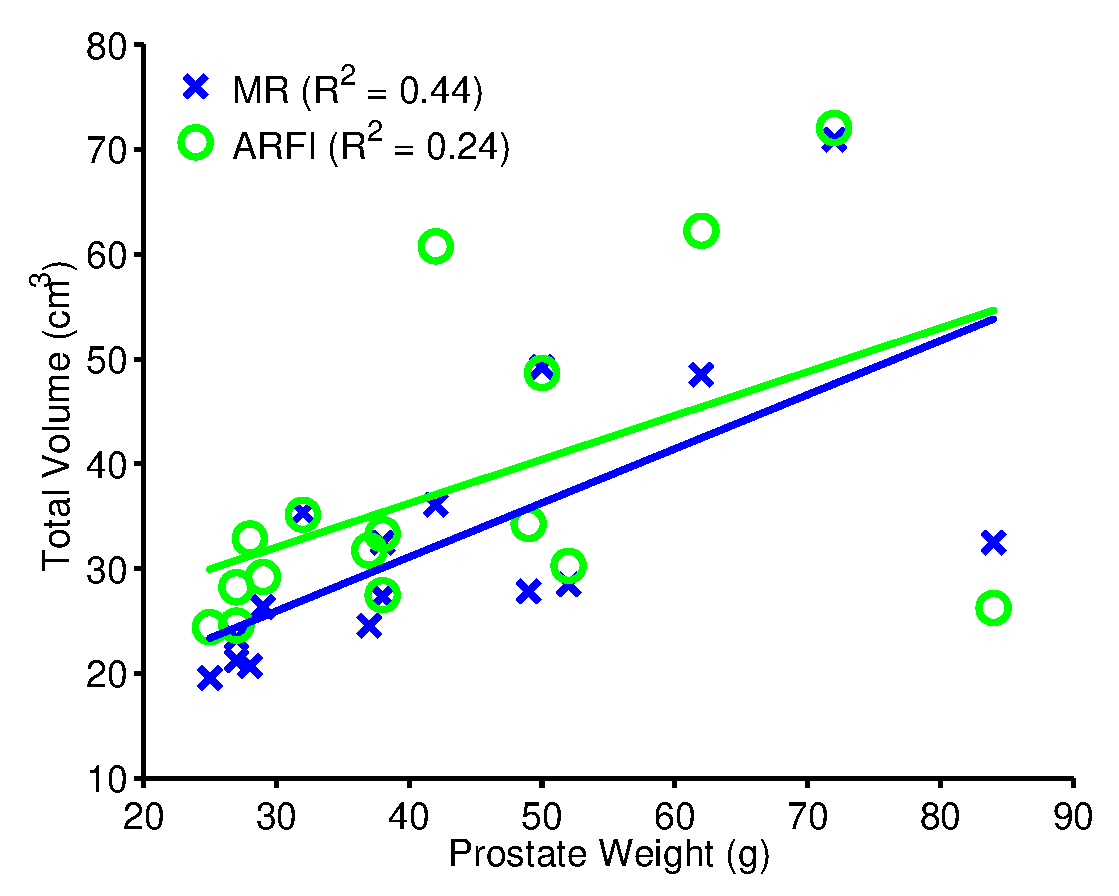
\includegraphics[width=0.3\linewidth]{figs/corr_weight_vol} &
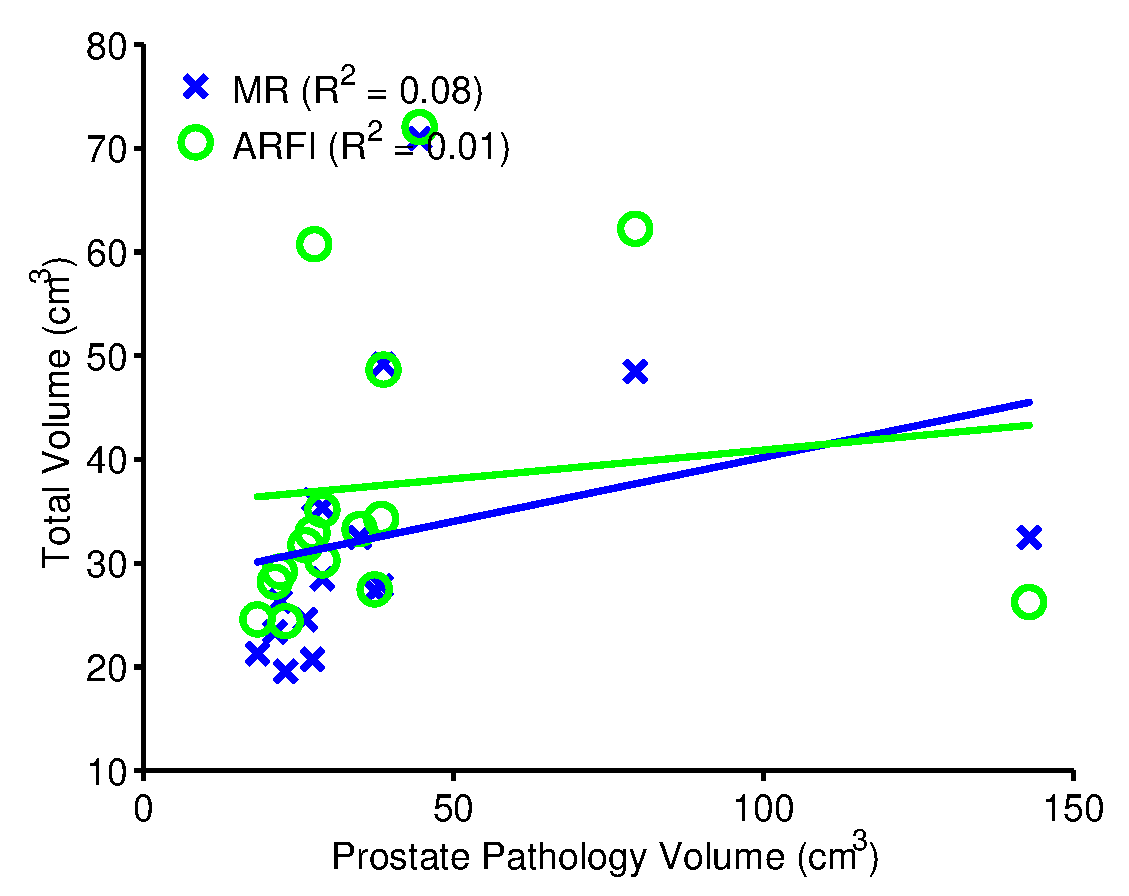
\includegraphics[width=0.3\linewidth]{figs/corr_pathVol_vol} \\
(a) Path Weight : Path Volume & (b) Image Volume : Prostate Weight & (c) Image Volume : Path Volume \\
\end{tabular}
\begin{tabular}{ll}
\includegraphics[width=0.3\linewidth]{figs/corr_weight_vol_no4} &
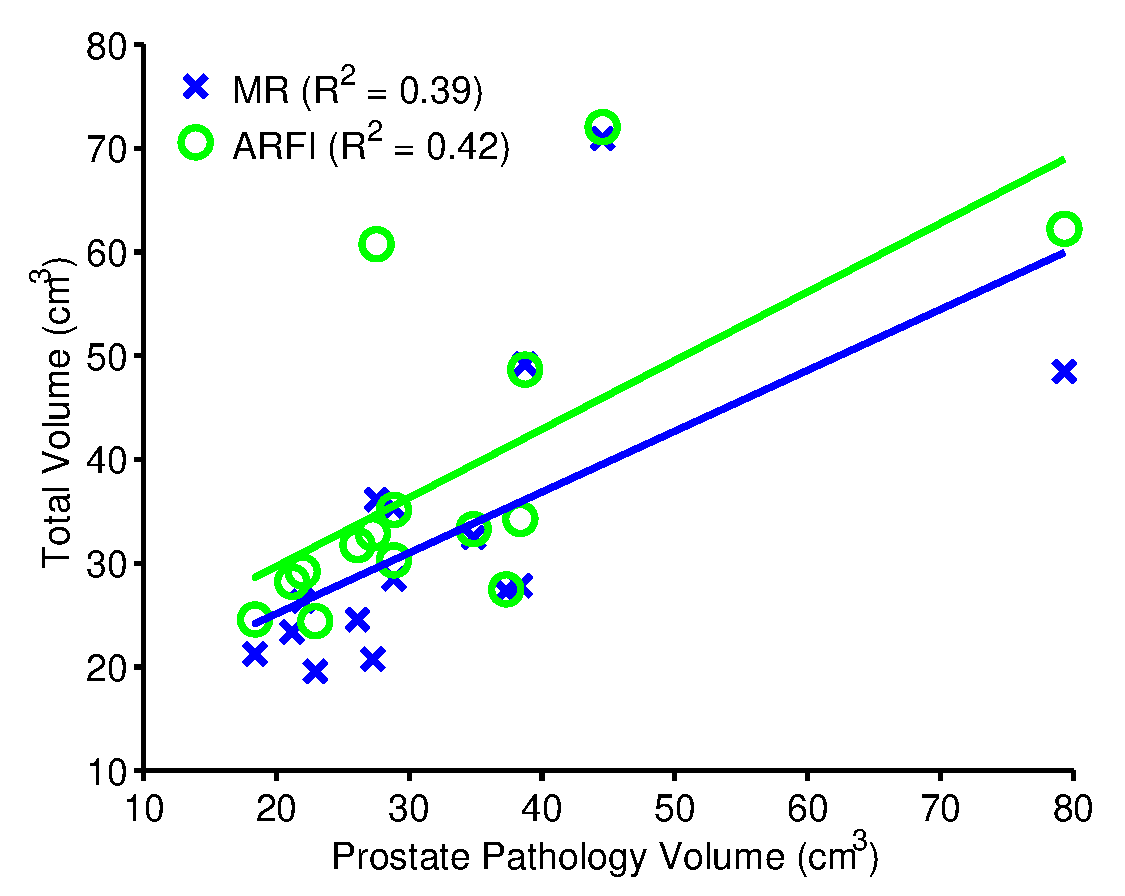
\includegraphics[width=0.3\linewidth]{figs/corr_pathVol_vol_no4} \\
(d) Image Volume : Prostate Weight (-4) & (e) Image Volume : Path Volume (-4) \\
\end{tabular}
\caption{Tri-axial pathology measurements were used to make an ellipsoidal
    prostate volume approximation based on gross pathology axis measurements,
    which was moderately well-correlated with the excised prostated weights (a,
    R$^2$ = 0.68).  T2WI MR (blue, X) showed a moderate correlation between the
    reconstructed volumes and prostate weight (R$^2$ = 0.44), while volumes
    reconstructed from ARFI images (green, O) showed weaker correlation (R$^2$
    = 0.21) (b).  Even weaker correlations existed between both T2WI MR and
    ARFI image volumens and approaximated ellipsoidal prostate pathology
    volumes (R$^2$ = 0.08 and 0.01, respectively) (c).  It should be noted in
    these figures that Study Subject 4 had an excessively large prostate that
    was difficult to fully capture in imaging, and was therefore grossly
    underestimated in size.  We retrospectively excluded that study subject
    from the analysis and re-calculated the coefficients of determination,
    showing that MR and ARFI imaging improved to R$^2$ = 0.74 and 0.60,
    respectively, for prostate weight (d), and R$^2$ = 0.39 for both imaging
    modalities relative to pathology gross volume (e).}
\label{fig:mr_arfi_weight}
\end{figure}
